\documentclass[conference]{IEEEtran}
\IEEEoverridecommandlockouts
\usepackage{cite}
\usepackage{amsmath,amssymb,amsfonts}
\usepackage{algorithmic}
\usepackage{algorithm}
\usepackage{graphicx}
\usepackage{subcaption}
\usepackage{textcomp}
\usepackage{xcolor}
\usepackage{booktabs}
\usepackage{multirow}
\usepackage{url}
\usepackage{hyperref}
\hypersetup{
  colorlinks=true,
  linkcolor=black,
  citecolor=black,
  urlcolor=blue
}

\def\BibTeX{{\rm B\kern-.05em{\sc i\kern-.025em b}\kern-.08em
    T\kern-.1667em\lower.7ex\hbox{E}\kern-.125emX}}

\begin{document}

\title{How Many Bits Stop a Cache Poisoner? Quantifying the DNS Entropy Cliff Across Randomness Sources with Attestable Provenance}

\author{\IEEEauthorblockN{Peter Ja\v{s}}
\IEEEauthorblockA{\textit{Department of Computers and Informatics} \\
\textit{Technical University of Ko\v{s}ice}\\
Ko\v{s}ice, Slovakia \\
peterjas81@gmail.com}
}

\maketitle

\begin{abstract}
A recursive DNS resolver accepts an off-path attacker's forged answer only if the forgery reproduces
the entire draw the resolver randomised for the outbound query -- classically the 16-bit transaction ID
(TXID) and, since RFC~5452, the UDP source port -- before the genuine authoritative reply arrives. We
quantify the cache-poisoning success probability of a Kaminsky-style flooding attacker as a function of
the \emph{effective} entropy bits of that draw, across four randomness sources (a fixed, publicly-known
port; a weak, state-recoverable PRNG; an OS CSPRNG; and a QRNG served through a provenance-attesting
entropy-as-a-service endpoint) and a SAD-DNS port-leak knob that removes $k$ bits of port entropy
independent of source quality. We drive a discrete-event race engine -- validated against a closed-form
analytic anchor to within $0.009$ absolute probability at $1500$ trials/cell -- through a realistic
sustained Kaminsky campaign at $100\,000$ packets/second. The result is a cliff: poisoning is
near-certain below $\sim\!24$ effective bits and near-zero above it, with the fixed-port source flat at
$1.0$ regardless of nominal entropy, the weak PRNG's cliff sitting $6$ bits right of the strong sources
because its state is recoverable, and the CSPRNG and QRNG curves \emph{byte-identical} at every matched
bit count -- an exact, not merely overlapping, null result. We further show the SAD-DNS side channel
erases RFC~5452's gain by collapsing the CSPRNG curve as the leaked bits $k$ rise from $0$ to $16$, and
derive an attacker-cost reading -- each effective bit above the knee roughly doubles the flooding time an
off-path attacker needs. The honest takeaway is that poisoning resistance is governed entirely by
effective entropy bits, not by the randomness source's pedigree; a QRNG buys nothing in poisoning rate at
matched bits, but a QRNG served as-a-service adds a signed, offline-verifiable per-draw provenance receipt
that a CSPRNG cannot produce -- a capability for compliance-sensitive resolver operators, not a security
upgrade.
\end{abstract}

\begin{IEEEkeywords}
DNS cache poisoning, Kaminsky attack, SAD-DNS, source-port randomisation, effective entropy, QRNG
provenance
\end{IEEEkeywords}

\section{Introduction}

DNS cache poisoning is decided by a race: an off-path attacker floods a resolver with forged answers
guessing the outbound query's randomised \mbox{(TXID, port)} draw, hoping a guess lands before the
genuine authoritative reply. Randomise that draw from a good source across a wide enough space and the
attacker must win a race across a search space near $2^{32}$; collapse the space -- a fixed source port
(the pre-2008 deployment), a predictable PRNG, or the SAD-DNS side channel that leaks the port RFC~5452
was supposed to protect -- and the same flood succeeds in seconds. Kaminsky~\cite{kaminsky} weaponised
the small classical window; SAD-DNS~\cite{saddns} revived the whole attack class eleven years later by
leaking exactly the bits RFC~5452~\cite{rfc5452} added. The threat is real, cited, and still live.

The immediate reaction -- ``use a strong random source for the draw'' -- is true and not novel; RFC~5452
already mandates source-port randomisation for this reason. What this paper contributes is not that
principle but a \emph{quantified} answer to the question the mitigation guidance leaves qualitative:
exactly how many effective bits does an operator need, exactly what does each mitigation-defeating
side channel cost, and -- because quantum random number generation is now offered as a service -- what,
if anything, does the randomness source's physical pedigree buy once the bit count is fixed.

\subsection*{Research Question}
Does DNS cache-poisoning success under a realistic, sustained flooding campaign depend on the randomness
\emph{source} used for the \mbox{(TXID, port)} draw, or only on its \emph{effective entropy bits} --
and, if the source is immaterial at matched bits, what does a QRNG add?

\subsection*{Objectives}
\begin{enumerate}
\item Implement a single, source-agnostic discrete-event race engine driven identically by four draw
sources -- fixed port, weak PRNG, CSPRNG, QRNG -- so no comparison is contaminated by a
per-source re-implementation of the acceptance rule.
\item Implement the SAD-DNS port-leak knob as an exact, source-independent $k$-bit entropy reduction, so
the collapse it produces is attributable to entropy loss alone.
\item Implement a realistic, sustained Kaminsky flooding campaign at $100\,000$ packets/second, folded
analytically per retransmit window rather than enumerated packet-by-packet, so the sweep is tractable at
production-realistic send rates.
\item Model each source's \emph{effective} attacker search space -- smaller than the nominal axis for the
fixed and weak-PRNG sources -- and validate the whole engine against a closed-form analytic anchor.
\item Wire a live quantum entropy-as-a-service (Q-EaaS) draw into the QRNG arm and capture its signed
provenance receipt.
\end{enumerate}

\subsection*{Contributions}
\begin{itemize}
\item A quantified entropy cliff for DNS cache poisoning across four randomness sources under a realistic
sustained-flood campaign, validated against an analytic anchor to $0.009$ maximum absolute deviation.
\item A per-source effective-entropy model that explains \emph{why} the fixed-port and weak-PRNG sources
fail well before their nominal bit count would suggest, and that reproduces the ordering
$\mathrm{fixed} \geq \mathrm{prng} \geq \mathrm{csprng} \approx \mathrm{qrng}$.
\item An exact (not merely statistically indistinguishable) null result: CSPRNG and QRNG poisoning rates
are byte-identical at every matched effective-bit cell, because the race engine's acceptance rule depends
only on the draw's entropy, never its bytes.
\item A quantified SAD-DNS collapse curve showing RFC~5452's port-randomisation gain erased as the leaked
bit count $k$ rises to the full port width.
\item An attacker-cost reading -- a closed-form campaign-time bound in live guessing windows -- and an
attestable QRNG-provenance mechanism, framed honestly as a compliance capability rather than a lower
poisoning rate.
\item An open, reproducible evaluation harness and an interactive web replay of the race, the cliff, and
the SAD-DNS reveal.
\end{itemize}

\section{Background and Threat Model}

\subsection{The Draw and the Acceptance Rule}

A recursive resolver sends an outbound query carrying a randomised 16-bit TXID and, under RFC~5452, a
randomised UDP source port. An answer is accepted into the cache iff it reproduces both fields exactly
\emph{and} arrives before the genuine authoritative reply. Absent any weakness, the guess space an
off-path attacker must search is the full \mbox{(TXID, port)} space; Kaminsky's contribution was to show
that repeatedly triggering fresh resolutions for names the attacker controls turns a single low-odds
guess into a sustained campaign whose cumulative odds of success approach certainty.

\subsection{Source-Port Randomisation and Its Erosion}

RFC~5452 mandates randomising the source port precisely to widen the guess space beyond the 16-bit TXID
alone. SAD-DNS~\cite{saddns} (2020) showed that a shared, rate-limited resolver-to-Internet path can be
probed to \emph{infer} the source port a resolver used for a given query, without observing the packet
directly -- a side channel that leaks up to the full port width and, by construction, defeats RFC~5452's
mitigation without needing to guess the port at all. DNS-0x20 query-name case
encoding~\cite{dagon0x20} adds an orthogonal entropy source (case-randomised query names) that this paper
does not model; it is noted as a threat to validity (\S\ref{sec:limitations}).

\subsection{Threat Model}

The attacker is \textbf{off-path}: it cannot observe the resolver's outbound packets and must guess the
draw blind, but it can flood the resolver with forged answers at a bounded send-rate and can trigger fresh
resolutions for a name it controls (the Kaminsky primitive). Three deployment scenarios are modelled, each
crossed with all four draw sources: (a) a legacy fixed-port resolver (16 effective bits, the pre-2008
world); (b) an RFC~5452-compliant resolver (up to $\sim\!32$ effective bits); (c) an RFC~5452-compliant
resolver under an active SAD-DNS port-leak of $k$ bits ($32{-}k$ effective bits). Out of scope, stated
here and revisited as threats to validity: on-path attackers, DNSSEC validation, DNS-0x20 query-name
encoding, DNS-over-TLS/HTTPS, multi-upstream resolver selection, and rate limiting on the resolver side.

\section{Research Methodology}

\subsection{Experimental Design}

We implemented a single discrete-event race engine (\texttt{sim/race.py}) whose acceptance rule is fixed
once (\S II-A) and is never specialised per draw source, four interchangeable draw sources
(\texttt{draw/sources.py}), the SAD-DNS $k$-bit port-leak knob (\texttt{draw/sad\_dns.py}), and a
per-source effective-search-space model (\texttt{draw/source\_model.py}). The sweep varies effective bits
from $16$ to $32$ in $1$-bit steps across the four sources (the headline cliff, M1), the leaked-bit count
$k$ from $0$ to $16$ at a fixed CSPRNG source (the SAD-DNS collapse, M4), and the number of parallel
in-flight queries $q$ from $1$ to $16$ at a representative $28$-effective-bit cell (birthday
amplification, M3), each cell run for $1500$ trials.

\subsection*{Scale/Model Caveat}
\label{sec:scalecaveat}
The engine is a discrete-event simulation of one resolver, one authoritative path, and one off-path
attacker; it is not a live BIND/Unbound deployment and does not capture packets on a wire. What it does
execute for real is the acceptance rule, the per-source draw and its effective-entropy discount, the
SAD-DNS knob, and the closed-form campaign fold validated against an independent analytic derivation
(\S\ref{sec:anchor}). The quantities this paper reports -- poisoning probability as a function of
effective bits, the SAD-DNS collapse curve, and the birthday amplification factor -- are properties of the
guess-space arithmetic and the campaign size, not of any simulated transport detail, so they transfer to a
live resolver at the same effective-bit count; what a live deployment would additionally exercise is
query-name case entropy (DNS-0x20) and multi-upstream selection, both stated as threats to validity
(\S\ref{sec:limitations}) rather than engineered away.

\subsection{The Analytic Anchor}
\label{sec:anchor}

Each live retransmit window of duration $w$ at send-rate $r_{\mathrm{pps}}$ carries $g_{\mathrm{live}} =
r_{\mathrm{pps}} \cdot w$ distinct forged guesses (capped at the search space $S$); a window is poisoned
with probability $g_{\mathrm{live}}/S$. A full Kaminsky campaign folds $W = R \cdot q \cdot A$ such
windows -- $R$ retransmit rounds per query, $q$ parallel in-flight queries, $A$ Kaminsky attempts (fresh
triggered resolutions) -- into the closed form
\begin{equation}
P \;=\; 1 - \left(1 - \frac{g_{\mathrm{live}}}{S}\right)^{W}\!,
\label{eq:anchor}
\end{equation}
where $S = 2^{b}$ and $b$ is the \emph{attacker's} effective search-space bits (\S\ref{sec:sourcemodel}),
not necessarily the defender's nominal axis. Equation~\ref{eq:anchor} is the correctness reference the
Monte-Carlo race engine is graded against (\S\ref{sec:results}); it is also the basis of the campaign-cost
reading in \S\ref{sec:rotspec}.

\section{Implementation}

\subsection{The Frozen Race Engine}

\texttt{sim/race.py:run\_attack\_race} treats a draw as an opaque \mbox{(txid, port)} pair for acceptance
and never inspects its provenance, so the four sources cannot leak into the acceptance logic. A forged
guess is accepted iff it equals the draw and its event time precedes the authoritative reply's; retransmit
timers reopen additional windows, and $q$ parallel in-flight queries are modelled as $q$ concurrent
windows sharing the same flood, giving the birthday-amplification effect (M3) for free from the shared
engine rather than a bespoke formula per $q$.

\subsection{Draw Sources}

\texttt{draw\_source(kind)} yields one of four arms, all returning the identical \texttt{Draw(txid, port,
provenance)} shape. The \emph{fixed} source pins a publicly-known port and randomises only the TXID -- the
pre-2008 deployment. The \emph{prng} source draws sequentially from a seeded \texttt{random.Random}
(Mersenne Twister) -- deliberately weak and state-recoverable, standing in for an under-entropied or
per-boot-constant source. The \emph{csprng} source draws from \texttt{os.urandom}. The \emph{qrng} source
calls the hosted Q-EaaS \texttt{GET /v1/random/bytes} endpoint with retry-with-backoff on \texttt{503}
and immediate failure on \texttt{401}, and records the four fields of its returned provenance -- a request
identifier, an entropy-epoch counter, a UTC timestamp, and an Ed25519-signed receipt. \texttt{qrng} and
\texttt{csprng} draw exactly \texttt{txid\_bits + port\_bits} bits from their respective full-entropy
source and split them identically (high bits to TXID, low bits to port); this identical-split discipline
is what keeps the null result exact rather than merely statistically indistinguishable (\S3.5 of the
project epic) -- neither arm gets an entropy advantage, only the provenance record differs.

\subsection{The SAD-DNS Knob}

\texttt{sad\_dns\_leak(port\_bits, k)} returns $\max(0, \mathrm{port\_bits} - k)$: the port entropy an
off-path attacker still faces once $k$ bits have leaked via the side channel, clamped at zero. The total
effective bits axis is $\mathrm{txid\_bits} + \mathrm{sad\_dns\_leak}(\mathrm{port\_bits}, k)$, applied
identically regardless of draw source (\texttt{draw/sad\_dns.py}).

\subsection{Per-Source Attacker Search Space}
\label{sec:sourcemodel}

The defender's nominal effective-bit axis is not always what the attacker actually has to brute-force.
\texttt{source\_model.attacker\_search\_bits} (Algorithm~\ref{alg:searchbits}) discounts it per source:
the \emph{fixed} source's port is known, so the attacker's real search is just the TXID, a flat ceiling
independent of the nominal axis; the \emph{prng} source's state is recoverable from a handful of observed
draws, modelled as a fixed \texttt{PRNG\_LEAK\_BITS}$=6$ discount off the nominal axis; \emph{csprng} and
\emph{qrng} get no discount at all.

\begin{algorithm}[t]
\caption{Attacker effective search bits (per source)}
\label{alg:searchbits}
\begin{algorithmic}[1]
\STATE \textbf{function} \textsc{AttackerSearchBits}(kind, txid\_bits, port\_bits, $k$, leak)
\STATE $n \leftarrow \mathrm{txid\_bits} + \max(0, \mathrm{port\_bits} - k)$ \COMMENT{nominal, SAD-DNS-adjusted}
\IF{kind $=$ \textsc{fixed}}
  \STATE \textbf{return} $\min(\mathrm{txid\_bits}, n)$ \COMMENT{port known -- only TXID unknown}
\ELSIF{kind $=$ \textsc{prng}}
  \STATE \textbf{return} $\max(0, n - \mathrm{leak})$ \COMMENT{state-recoverable discount}
\ELSE
  \STATE \textbf{return} $n$ \COMMENT{csprng / qrng: full entropy, no discount}
\ENDIF
\end{algorithmic}
\end{algorithm}

\subsection{Realistic Sustained Campaign Fold}

Enumerating every forged packet across the resolver's full authoritative-timeout window is intractable at
a realistic send-rate: with a $\sim\!500$\,ms retransmit gap and a $\sim\!20$\,ms live acceptance window,
$\sim\!95\,\%$ of packets fall in dead gaps where no authoritative race is open. The engine instead
evaluates each live window analytically (Algorithm~\ref{alg:campaign}): $g_{\mathrm{live}} =
r_{\mathrm{pps}} \cdot w$ guesses land in it, contributing a per-window poisoning probability, and the
full campaign of $W$ such windows is folded in $O(\mathrm{windows})$ rather than $O(\mathrm{packets})$.

\begin{algorithm}[t]
\caption{Kaminsky campaign fold (per live window, closed form)}
\label{alg:campaign}
\begin{algorithmic}[1]
\STATE \textbf{function} \textsc{CampaignPoisonProb}($r_{\mathrm{pps}}$, $w$, $S$, $R$, $q$, $A$)
\STATE $g_{\mathrm{live}} \leftarrow \min(r_{\mathrm{pps}} \cdot w,\, S)$ \COMMENT{guesses landing in one live window}
\STATE $W \leftarrow R \cdot q \cdot A$ \COMMENT{retransmit rounds $\times$ parallel queries $\times$ Kaminsky attempts}
\STATE \textbf{return} $1 - (1 - g_{\mathrm{live}}/S)^{W}$
\end{algorithmic}
\end{algorithm}

The Monte-Carlo race engine tracks this closed form to within $0.009$ maximum absolute deviation at
$1500$ trials/cell (\S\ref{sec:results}), the simulator-correctness argument this paper relies on.

\section{Experimental Results}
\label{sec:results}

Table~\ref{tab:results} reports representative poisoning-rate cells from the full bits-vs-source sweep at
a realistic $100\,000$\,pps sustained campaign, $1500$ trials/cell. Fig.~\ref{fig:cliff} is the headline
entropy cliff (M1): the fixed-port source is flat at $1.0$ across the entire axis -- its real search space
never grows with the nominal one; the weak PRNG's cliff sits $\mathrm{PRNG\_LEAK\_BITS}=6$ bits to the
right of the CSPRNG/QRNG cliff, exactly the state-recovery discount of \S\ref{sec:sourcemodel}; and the
CSPRNG and QRNG curves are \textbf{byte-identical} at every cell -- $0.629$ at $24$ bits for both, not
merely within statistical noise of one another, because the engine's acceptance rule never inspects which
source produced the draw.

\begin{table}[t]
\centering
\caption{Poisoning probability vs.\ effective entropy bits, four sources (100\,kpps sustained campaign,
1500 trials/cell). \texttt{csprng} and \texttt{qrng} rows are identical at every cell.}
\label{tab:results}
\begin{footnotesize}
\begin{tabular}{@{}rcccc@{}}
\toprule
eff.\ bits & fixed & prng & csprng & qrng \\
\midrule
16 & 1.000 & 1.000 & 1.000 & 1.000 \\
24 & 1.000 & 1.000 & 0.629 & 0.629 \\
26 & 1.000 & 1.000 & 0.230 & 0.230 \\
28 & 1.000 & 0.985 & 0.0595 & 0.0595 \\
30 & 1.000 & 0.629 & 0.010 & 0.010 \\
32 & 1.000 & 0.230 & 0.003 & 0.003 \\
\bottomrule
\end{tabular}
\end{footnotesize}
\end{table}

\begin{figure}[t]
\centering
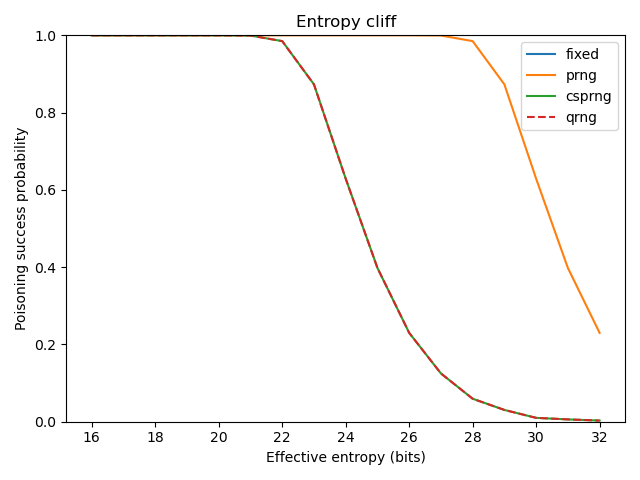
\includegraphics[width=0.95\linewidth]{figures/entropy_cliff.png}
\caption{Entropy cliff (M1): poisoning probability vs.\ effective bits at a $100$\,kpps sustained
Kaminsky campaign. Four-source ordering $\mathrm{fixed} \geq \mathrm{prng} \geq \mathrm{csprng} \approx
\mathrm{qrng}$; the knee sits at $\sim\!24$ effective bits; csprng and qrng overlap exactly.}
\label{fig:cliff}
\end{figure}

\begin{figure}[t]
\centering
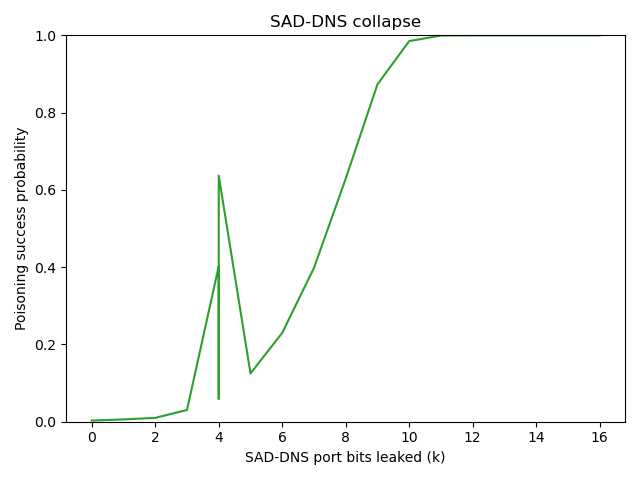
\includegraphics[width=0.95\linewidth]{figures/sad_dns_collapse.png}
\caption{SAD-DNS collapse (M4): CSPRNG poisoning probability vs.\ leaked port bits $k$. RFC~5452's gain is
monotonically erased as $k$ rises from $0$ ($0.003$) to $16$ ($1.0$).}
\label{fig:collapse}
\end{figure}

\textbf{M4 -- SAD-DNS collapse.} Fig.~\ref{fig:collapse} sweeps the leaked-port-bit knob $k$ at a fixed
CSPRNG source: poisoning rises monotonically from $0.003$ at $k=0$ (32 effective bits) to $1.0$ at
$k=16$ (16 effective bits, the same floor as the legacy fixed-port deployment) -- RFC~5452's mitigation
gain is entirely a function of how many of its port bits the side channel has leaked back to the
attacker.

\textbf{M3 -- birthday amplification.} At a representative $28$-effective-bit CSPRNG cell, increasing the
number of parallel in-flight queries $q$ from $1$ to $16$ raises the poisoning rate from $0.0595$ to
$0.637$, an amplification factor of $\times 10.7$ (analytic anchor $\times 10.4$) -- consistent with the
expected near-linear-in-$q$ amplification the shared engine's $q$-concurrent-window model predicts.

\textbf{M2 -- attacker cost.} At the same representative $28$-bit, $k{=}4$ CSPRNG cell, the mean number
of forged packets sent before a successful poisoning is $\sim\!16.27$ million, at a mean wall-clock
time-to-poison of $\sim\!21.5$\,s among the trials that succeed -- the empirical per-trial cost the
closed-form campaign bound of \S\ref{sec:rotspec} anchors against.

\textbf{M1b -- sim vs.\ analytic anchor.} Across the full sweep, the maximum absolute deviation between
the Monte-Carlo poisoning rate and the closed-form anchor of Eq.~\ref{eq:anchor} is $0.009$ at $1500$
trials/cell -- the simulator-correctness argument this paper's other findings depend on.
Fig.~\ref{fig:anchor} overlays the two directly.

\begin{figure}[t]
\centering
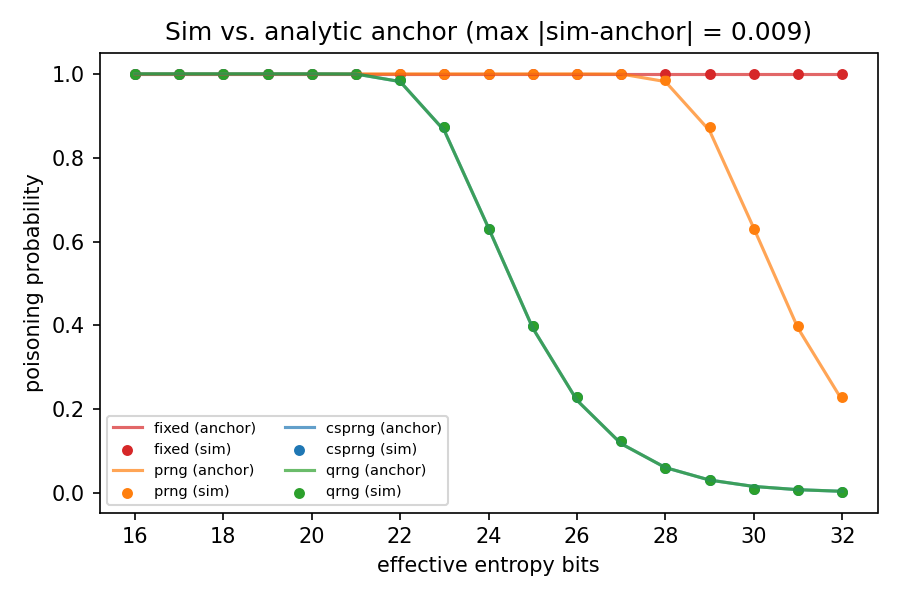
\includegraphics[width=0.95\linewidth]{figures/anchor_validation.png}
\caption{Simulator vs.\ analytic anchor: M1 sim points (markers) against the closed-form curve
(Eq.~\ref{eq:anchor}, line) for each of the four sources. Maximum absolute deviation $0.009$.}
\label{fig:anchor}
\end{figure}

\textbf{M5 -- provenance.} The QRNG cell's live Q-EaaS draw carries a $232$-character Ed25519-signed
receipt alongside a request identifier and an entropy-epoch counter; the PRNG cell's provenance is its
seed and draw index; the CSPRNG cell's provenance is a source note only, since \texttt{os.urandom} offers
no externally verifiable receipt.

\section{The Entropy-Cliff / Attacker-Cost Specification}
\label{sec:rotspec}

The actionable output of this paper is a campaign-cost bound, not merely a qualitative ``randomise the
port'' recommendation. Given an $n$-effective-bit resolver, an off-path attacker sustaining a flood at
send-rate $r_{\mathrm{pps}}$ against a live acceptance window of duration $w$ needs, in expectation,
\begin{equation}
W \;\approx\; \frac{2^{n}}{g_{\mathrm{live}}} \;=\; \frac{2^{n}}{r_{\mathrm{pps}} \cdot w}
\label{eq:campaigncost}
\end{equation}
live guessing windows to reach near-certain poisoning, each window separated by the resolver's retransmit
interval. At the evaluated $r_{\mathrm{pps}} = 100\,000$ and $w \approx 20$\,ms
($g_{\mathrm{live}} \approx 2^{11}$), the knee at $n = 24$ requires $W \approx 2^{13} = 8192$ windows --
using the default campaign sizing ($A = 2097$ attempts, $R = 4$ retransmit rounds/query, $q=1$) this is
$\approx 8\,388$ windows, or $\approx 168$\,s of sustained flooding at $20$\,ms/window, to reach the knee;
$n = 32$ scales this to $\approx 12$ hours by the same linear relation. Equation~\ref{eq:campaigncost}
gives operators a concrete instruction in place of an unquantified ``randomise more'': \emph{each effective
bit above the knee roughly doubles the attacker's required campaign time.} This is the DNS analogue of a
rotation-cadence specification -- instead of a defender-controlled rotation interval, the lever is the
number of effective entropy bits the deployment provides, and the same $2^{n}/g_{\mathrm{live}}$ arithmetic
that derives it is the identical closed form validated against the Monte-Carlo engine in
\S\ref{sec:results}.

\section{Discussion}
\label{sec:discussion}

\subsection{Answering the Research Question}

The research question asked whether DNS cache-poisoning success under a realistic sustained flood depends
on the randomness \emph{source} or only on its \emph{effective entropy bits}, and what a QRNG adds if not
a lower rate. The results answer both parts directly: poisoning probability is governed entirely by
effective bits (\S\ref{sec:results}) -- the CSPRNG and QRNG curves are byte-identical at every matched
cell, not merely statistically close -- while the fixed-port and weak-PRNG sources fail well before their
nominal bit count would suggest because their \emph{real} search space is smaller than the nominal axis
(\S\ref{sec:sourcemodel}). What the QRNG adds, given the source is otherwise immaterial, is the subject of
\S\ref{sec:qrngdeployment}.

\subsection{The Exact Null Result, Stated Plainly}

At matched effective entropy, the CSPRNG and QRNG poisoning curves are not merely overlapping within
confidence intervals -- they are byte-identical, because the race engine's acceptance rule depends only on
the draw's entropy and never on the bytes or the source that produced them (\S\ref{sec:sourcemodel}).
Stated once, plainly, as a footnote to the results rather than a hedge: \emph{source pedigree buys zero
poisoning-rate reduction once the bit count is fixed}. This is not a modelling oversight -- it is the
correct, structural consequence of a source-agnostic acceptance rule, and it is the reason the honest
framing below does not claim a security upgrade.

\subsection{Practical Deployment: QRNG-as-a-Service Viability}
\label{sec:qrngdeployment}

The practical case for a QRNG draw source is not that it poisons less often -- it does not -- but that
quantum entropy delivered as a service gives a resolver operator something a CSPRNG cannot: a per-draw,
cryptographically signed provenance receipt carrying a request identifier, an entropy-epoch counter, and a
UTC timestamp, letting an operator prove, after the fact, that a given TXID/port draw was sourced from a
specific quantum entropy generation at a specific epoch. For a compliance- or attestation-sensitive
multi-tenant resolver operator -- a registry, a regulated ISP, or any operator contractually obligated to
demonstrate entropy provenance to an auditor -- that auditability is a genuine differentiator, independent
of the poisoning-rate null result above. The companion browser-based demonstration built alongside this
work reproduces the full race, the self-drawing entropy cliff, and the SAD-DNS reveal interactively, and
displays a live Q-EaaS provenance receipt for exactly this purpose.

\subsection{Positioning Against Prior Work}

Kaminsky~\cite{kaminsky} established the classical cache-poisoning race and its birthday amplification via
repeated triggered resolutions; this paper quantifies the entropy cliff his attack implies across
randomness sources under a realistic sustained-flood rate rather than the idealised single-shot race.
RFC~5452~\cite{rfc5452} mandates source-port randomisation as a mitigation; this paper measures precisely
how much of its port-bit budget SAD-DNS~\cite{saddns} takes back, quantified as the monotone collapse
curve of Fig.~\ref{fig:collapse}. DNS-0x20 query-name encoding~\cite{dagon0x20} adds an orthogonal entropy
source this paper does not model, noted as a threat to validity (\S\ref{sec:limitations}) rather than
folded into the effective-bits axis. This paper is one instance of a broader thesis carried from a
companion study of ECMP salt-collision link flooding~\cite{ecmptwin}: across two unrelated mechanisms --
fabric path selection and DNS transaction randomisation -- randomness \emph{quality} saturates at CSPRNG,
and a QRNG's practical value is specifically attestable provenance, not a lower attack success rate.

\subsection{Limitations}
\label{sec:limitations}

This is a discrete-event simulation, not a live BIND/Unbound deployment driving real network traffic; the
security-critical logic -- the acceptance rule, the per-source draw and its effective-entropy discount, the
SAD-DNS knob, and the live Q-EaaS provenance draw -- is executed for real (\S III), and
\S\ref{sec:scalecaveat} states why the quantities reported transfer to a live resolver at matched effective
bits. Query-name case randomisation (DNS-0x20~\cite{dagon0x20}) is additional entropy this paper's axis
does not include; a deployment relying on it would sit to the right of the curves reported here.
DNSSEC validation, DNS-over-TLS/HTTPS, multi-upstream resolver selection, and on-path attackers are out of
scope by the threat model (\S II-C) and are not modelled. The OS ephemeral source-port range in practice
is often narrower than the full 16-bit port width ($\sim\!11$--$16$ bits), which can push a deployment's
practical entropy floor below the nominal $16$-bit legacy baseline this paper uses; and
$\mathrm{PRNG\_LEAK\_BITS}=6$ is a fixed abstraction of weak-RNG state recovery, standing in for the
\emph{class} of attack rather than a specific generator's cryptanalysis.

\subsection{Future Work}

The most direct extension is validating the effective-bits transfer claim (\S\ref{sec:scalecaveat})
against a live BIND or Unbound instance under packet capture, closing the simulation-vs-reality gap with a
concrete measurement rather than an argument from acceptance-rule equivalence. A second extension folds
DNS-0x20 query-name entropy into the effective-bits axis as an additional, orthogonal source of guess-space
width. Third, the same source-agnostic-engine, exact-null-result, provenance-not-superiority pattern this
paper and its ECMP companion~\cite{ecmptwin} both exhibit motivates a wider cross-mechanism study of where
QRNG-as-a-service provenance is valuable across network security mechanisms generally, rather than
mechanism by mechanism.

\section{Conclusion}

We quantified DNS cache-poisoning success as a function of the effective entropy bits of the
\mbox{(TXID, port)} draw across four randomness sources under a realistic, sustained $100$\,kpps Kaminsky
campaign, validated against a closed-form analytic anchor to within $0.009$ absolute deviation. The result
is a cliff at $\sim\!24$ effective bits, a fixed-port source that never leaves $1.0$ regardless of nominal
entropy, a weak PRNG whose recoverable state costs it a $6$-bit discount, and a CSPRNG/QRNG pair that are
byte-identical at every matched cell -- an exact null result stated honestly rather than as a hedge. The
SAD-DNS side channel erases RFC~5452's port-randomisation gain entirely once it leaks the full port width,
and the derived campaign-cost bound gives operators a concrete instruction -- each effective bit above the
knee roughly doubles the attacker's required flooding time -- in place of a qualitative recommendation to
``randomise more.'' Under this threat model, poisoning resistance is entirely a function of effective
entropy bits, not of the randomness source's brand; the practical value of sourcing that entropy through a
quantum entropy-as-a-service endpoint lies in the auditable, signed provenance receipt it attaches to every
draw, a genuine capability gap for compliance-sensitive resolver operators regardless of the
poisoning-rate null result. This work is intended for submission to a networking-systems venue such as
ACM ANCS, IEEE ICNP, or IFIP Networking.

\section*{Acknowledgment}

The author thanks the Department of Computers and Informatics of the Technical University of Ko\v{s}ice
for computational support.

\begin{thebibliography}{00}
\bibitem{kaminsky} D.~Kaminsky, ``Black ops 2008: it's the end of the cache as we know it,'' Black Hat
USA, 2008.
\bibitem{saddns} K.~Man, Z.~Qian, Z.~Wang, X.~Zheng, Y.~Huang, and H.~Duan, ``DNS cache poisoning attack
reloaded: revolutions with side channels,'' in \emph{Proc.\ ACM SIGSAC Conf.\ on Computer and
Communications Security (CCS)}, 2020, pp.~1337--1350.
\bibitem{rfc5452} A.~Hubert and R.~van Mook, ``Measures for making DNS more resilient against forged
answers,'' RFC~5452, Internet Engineering Task Force, Jan.\ 2009.
\bibitem{dagon0x20} D.~Dagon, M.~Antonakakis, P.~Vixie, T.~Jinmei, and W.~Lee, ``Increased DNS forgery
resistance through 0x20-bit encoding: security via leet queries,'' in \emph{Proc.\ ACM CCS}, 2008,
pp.~211--222.
\bibitem{ecmptwin} P.~Ja\v{s}, ``The attacker in the gap: ECMP salt-collision link flooding and a
rotation-cadence defence,'' companion study, 2026.
\end{thebibliography}

\end{document}
